\documentclass{beamer}

\usetheme{Antibes}

\usepackage[ngerman]{babel}
\usepackage[utf8x]{inputenc}
\usepackage{totpages}

\usepackage{listings}
\usepackage{epstopdf}

\setbeamercovered{transparent}
\beamertemplatenavigationsymbolsempty
%\setbeamertemplate{footline}[frame number]
\setbeamertemplate{footline}
  {%
    \begin{beamercolorbox}[ht=2.5ex,dp=1.125ex,%
      leftskip=.3cm,rightskip=.3cm plus1fil]{upper separation line foot}
       \hfill Folie~\thepage / \ref{TotPages}
    \end{beamercolorbox}
    \begin{beamercolorbox}[ht=2.5ex,dp=1.125ex,%
      leftskip=.3cm,rightskip=.3cm plus1fil]{author in head/foot}%
      \leavevmode{\usebeamerfont{author in head/foot}\insertshortauthor}%
      \hfill%
      {\usebeamerfont{institute in head/foot}\usebeamercolor[fg]{institute in 						head/foot}\insertshortinstitute}%
    \end{beamercolorbox}%
    \begin{beamercolorbox}[colsep=1.5pt]{lower separation line foot}	
    \end{beamercolorbox}
  }
  
\title{Asymmetrische Kryptographie in Java}
\subtitle{Sichere verteilte Anwendungen mit Java}
\author{A. H. W. Lindemann, N. Vetter}
\date{10. Januar 2014}

\institute[Universität Potsdam]{
	Institut für Informatik
}

\begin{document}

\begin{frame}
\titlepage
\end{frame}

\section{Übersicht}
\begin{frame}
\frametitle{Gliederung}
\tableofcontents
\end{frame}
\section{Theoretische Grundlagen}
\begin{frame}
\frametitle{Übersicht}
\begin{enumerate}
\item Übersicht
\item \textcolor{blue}{Theoretische Grundlagen}
\begin{itemize}
	\item Ziel
	\item Mathematische Grundlagen
	\item Vorstellung: Asymmetrische Kryptographie
	\item Vor-/Nachteile
\end{itemize}
\item Schlüsselmanagement
\item Java Cryptography Extension
\item Hybride Kryptographie
\item Demonstration
\item Literaturliste
\end{enumerate}
\end{frame}

\subsection*{Ziel}
\begin{frame}
\frametitle{Ziele}
\begin{itemize}
\item verbergen des Inhaltes einer Nachricht durch:
\begin{itemize}
\item Transformieren von Klartext in Kryptotext\\
\item späteres Entschlüsseln von Kryptotext in Klartext\\
\end{itemize}
\end{itemize}
\begin{block}{Kerckhoffs Prinzip:}
\glqq Sicherheit ist allein vom Schlüssel und nicht vom Verfahren abhängig.\grqq 
\end{block}
 
\end{frame}


\subsection*{Vorstellung: Asymmetrische Kryptographie}
\begin{frame}
\frametitle{Asymmetrische Kryptographie}
\begin{itemize}
\item entstand Mitte der 1970ger Jahre\\
\item von Ralph Merkle sowie Diffie und Hellmann entwickelt\\
\end{itemize}
Grundidee:
\begin{itemize}
\item öffentlicher und privater Schlüssel (Schlüsselpaar)
\end{itemize}
Anforderungen:
\begin{itemize}
\item Schlüssel müssen leicht zu generieren sein
\item privater Schlüssel darf nicht unter vertretbarem Aufwand aus öffentlichen Schlüssel zu berechnen sein
\item Ver- und Entschlüsselung müssen effizient berechenbar sein
\end{itemize}
\end{frame}

\subsection*{Mathematische Grundlagen}
\begin{frame}
\frametitle{Ansatz}
\hspace{12mm}$\Rightarrow$ Einwegfunktionen.
Definition:
\begin{itemize}
\item injektive Funktion $f:X \rightarrow Y$
\item $\forall x \in X$ ist f(x) \glqq effizient\grqq \,zu berechnen
\item aus Bild y = f(x) darf Urbild x nicht effizient berechnet werden können
\item Bsp.: Faktorisierungsproblem, Diskreter Logarithmus
\end{itemize}
\end{frame}
\begin{frame}
\frametitle{Lösung}
\hspace{12mm}$\Rightarrow$ Einwegfunktionen mit Falltür.
\begin{itemize}
\item injektive Funktion $f:X \rightarrow Y$
\item $\forall x \in X$ ist f(x) effizient zu berechnen
\item aus Bild y = f(x) darf Urbild x nur \glqq effizient\grqq ~berechnet werden können, wenn Zusatzinformationen verfügbar sind.
\item Bsp.: h-te Potenz mod(n), Zusammengesetzter mod(n)
\end{itemize}
\end{frame}

\begin{frame}
\frametitle{Bestandteile}
\begin{itemize}
\item Tupel = ($M,C,EK,DK,E,D$)
\item 2 endliche Alphabete ($A_1,A_2$)
\item Klartext ($M \subseteq A^*_1\backslash\emptyset$)
\item Kryptotext ($C \subseteq A^*_2\backslash\emptyset$)
\item Verschlüsselungsschlüsselraum ($EK\backslash\emptyset$)
\item Entschlüsselungsschlüsselraum\\
($DK/\emptyset~mit~f:EK \rightarrow DK ~und~ f(K_E)=K_D)$
\item Verschlüsselungsverfahren ($E :~ M x EK \rightarrow C$)
\item Entschlüsselungsverfahren ($D :~ C x DK \rightarrow M$)
\item Es gilt: $\forall M : D(E(M,K_E),K_D) = M$
\end{itemize}
\end{frame}
\begin{frame}
\frametitle{Erläuterung}
\hspace*{-1cm}
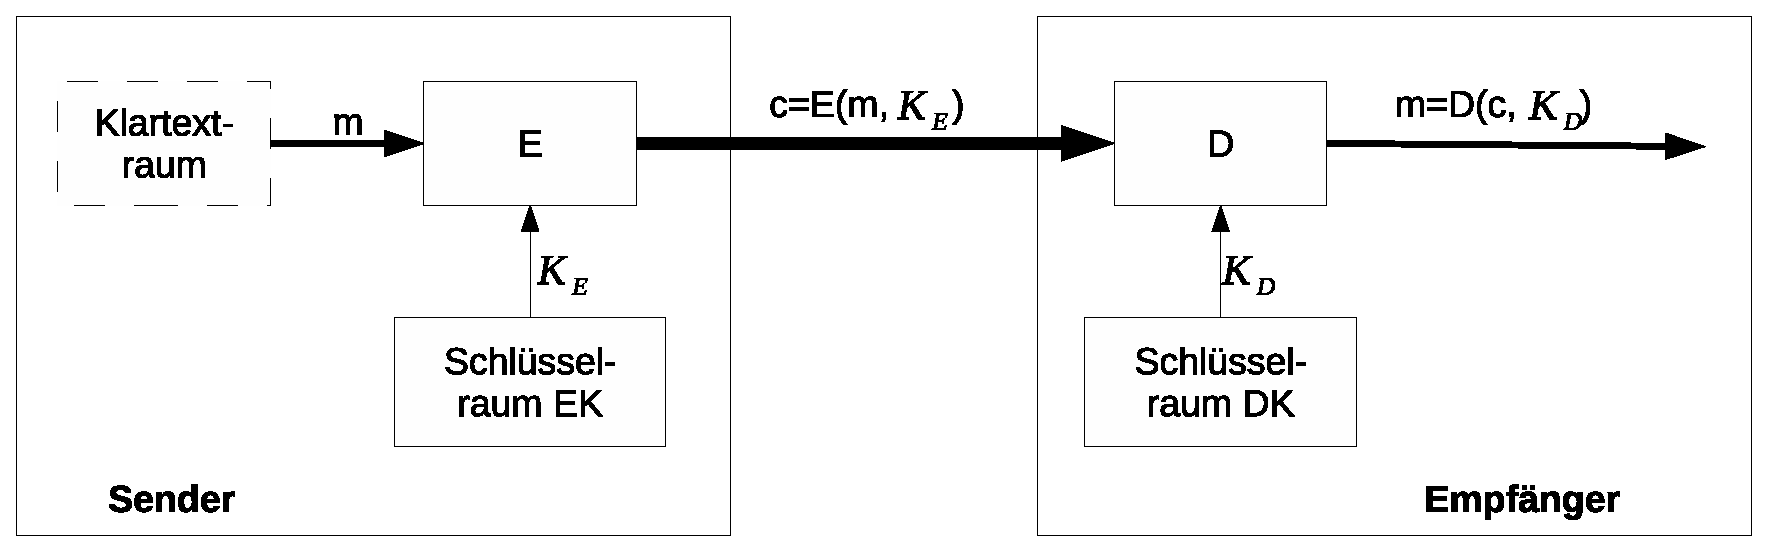
\includegraphics[width=\paperwidth]{async.eps}

(nach Eckert\cite{Eckert13})
\end{frame}

\begin{frame}
\frametitle{Vertreter}
\begin{itemize}
\item RSA
\item Diffie-Hellman
\item DSA
\item ElGamal
\end{itemize}

\begin{block}{Findet Anwendung bei:}
\begin{itemize}
\item PGP
\item SSL/TLS (SSH, HTTPS, ...)
\end{itemize}
\end{block}
\end{frame}

\subsection*{Vor-/Nachteile}
\begin{frame}
\frametitle{Vor-/Nachteile}
Vorteil:
\begin{itemize}
\item kein Schlüsselaustausch notwendig
\end{itemize}
Nachteil:
\begin{itemize}
\item hohe Komplexität der Berechnungen\\ $\rightarrow$ unter Umständen langsam
\item Authentizität des öff. Schlüssels nicht garantiert 
\\$\rightarrow$ \glqq man in the middle\grqq
\end{itemize} 
\end{frame}

\section{Schlüsselmanagement}
\begin{frame}
\frametitle{Übersicht}
\begin{enumerate}
\item Übersicht
\item Theoretische Grundlagen
\item \textcolor{blue}{Schlüsselmanagement}
\begin{itemize}
	\item Erzeugung von Schlüsselmaterial
	\item Schlüsselspeicherung
	\item Schlüsselwiederherstellung
\end{itemize}
\item Java Cryptography Extension
\item Hybride Kryptographie
\item Demonstration
\item Literaturliste
\end{enumerate}
\end{frame}

\subsection*{Erzeugung von Schlüsselmaterial}
\begin{frame}
\frametitle{Erzeugung}
2 Möglichkeiten zur Erzeugung:
\begin{itemize}
\item Nutzer erzeugt Schlüsselpaar selbst 
\\(oder lässt ein Token ein Schlüsselpaar erzeugen)
\begin{itemize}
\item Nutzer hat volle Kontrolle über den Prozess
\item Verantwortung liegt allein beim Nutzer
\\(Aufbewahrung, Sicherung, ...)
\item heterogene Umgebung zur Generierung
\end{itemize}
\item zentrale Instanz stellt Schlüsselpaar bereit (z.B. CA)
\begin{itemize}
\item Nutzer hat keine volle Kontrolle über den Prozess
\item Schlüsselmaterial kann gesichert werden 
\\(siehe Schlüsselwiederherstellung)
\item Transport des Schlüsselpaares kritisch
\end{itemize}
\end{itemize} 
\end{frame}
\subsection*{Schlüsselspeicherung}
\begin{frame}
\frametitle{Speicherung und Verbreitung}
Ansatz:
\begin{itemize}
\item keine Instanz außer dem Besitzer darf den priv. Schlüssel einsehen (am besten nicht mal dieser) 
\item öffentlicher Schlüssel soll frei verfügbar sein
\end{itemize}
Möglichkeiten:
\begin{itemize}
\item privater Schlüssel:
\begin{itemize}
\item selbst sicher gespeichert
\item zentrale Instanz
\item Token (Bsp.: SmartCard)
\end{itemize}
\item öffentlicher Schlüssel:
\begin{itemize}
\item Verteilen per E-Mail oder ähnliches
\item zentrale Instanz
\end{itemize}
\end{itemize}
\end{frame}
\subsection*{Schlüsselwiederherstellung}
\begin{frame}
\frametitle{Wiederherstellung}
Nur möglich durch Speicherung des priv. Schlüssels \\(oder Schlüsselmaterials)\\
Vorteile:
\begin{itemize}
\item keine neue Verteilung des öff. Schlüssels notwendig
\item Wiederherstellung der verschlüsselten Daten
\end{itemize}
Nachteile:
\begin{itemize}
\item Schlüsselbackup ist zentraler Angriffspunkt 
\end{itemize}
\end{frame}

\section{Java Cryptography Extension}
\begin{frame}
\frametitle{Übersicht}
\begin{enumerate}
\item Übersicht
\item Theoretische Grundlagen
\item Schlüsselmanagement
\item \textcolor{blue}{Java Cryptography Extension}
\begin{itemize}
	\item Java Cryptography Architecture
	\item Kryptoprovider
\end{itemize}
\item Hybride Kryptographie
\item Demonstration
\item Literaturliste
\end{enumerate}
\end{frame}

\subsection*{Java Cryptography Architecture}
\begin{frame}
\frametitle{JCA vs JCE}
\begin{itemize}
\item \textcolor{blue}{\textbf{J}ava \textbf{C}ryptography \textbf{A}rchitecture} - Hashfunktionen, Schlüsselgeneratoren,...
\item \textcolor{blue}{\textbf{J}ava \textbf{C}ryptography \textbf{E}xtension} - Verschlüsselungsfunktionen
\item Abspaltung aufgrund von Exportbeschränkungen der USA
\end{itemize}
\end{frame}

\subsection*{Kryptoprovider}
\begin{frame}
\frametitle{Integrierte Provider}
\framesubtitle{The SunJCE Provider}
Fähigkeiten (unter anderem):
\begin{itemize}
\item AES, DES, ...
\item RSA
\item Diffie-Hellman
\end{itemize}
\end{frame}

\begin{frame}[fragile]
\frametitle{Externe Provider}
\framesubtitle{Bouncy Castle}
Aktivierung zur Laufzeit:
\begin{lstlisting}[frame=shadowbox]
 Security
 	.addProvider( new BouncyCastleProvider() );
\end{lstlisting}
systemweite dauerhafte Aktivierung:
\begin{itemize}
\item Eintrag in die Datei: \$JAVA/lib/security/java.security\\
(\$JAVA = Pfad zum Java Runtime Environment)
\end{itemize}

\begin{block}{Fähigkeiten (unter anderem):}

\begin{itemize}
\item AES, DES, ...
\item RSA, ElGamal, NTRU
\item Diffie-Hellman (verschiendene Varianten)
\end{itemize}
\end{block}
\end{frame}


\section{Hybride Kryptographie}
\begin{frame}
\frametitle{Übersicht}
\begin{enumerate}
\item Übersicht
\item Theoretische Grundlagen
\item Schlüsselmanagement
\item Java Cryptography Extension
\item \textcolor{blue}{Hybride Kryptographie}
\begin{itemize}
	\item Vorstellung
	\item Implementierung
\end{itemize}
\item Demonstration
\item Literaturliste
\end{enumerate}
\end{frame}

\subsection*{Vorstellung}
\begin{frame}
\frametitle{Hybride Kryptographie}
\hspace*{-1cm}
\includegraphics[width=\paperwidth]{hybrid.PNG} 

\hspace*{-0.5cm}
(aus VL "`Sicherheit in Rechnernetzen"' bei Prof. Dr. Bettina Schnor)
\end{frame}

\begin{frame}
\frametitle{Hybride Kryptographie}

Mischung aus symmetrischer und asymmetrischer Kryptographie:
\begin{itemize}
	\item Nachricht wird symmetrisch verschlüsselt
	\item symmetrischer Schlüssel wird asymmetrisch verschlüsselt
	\item Nachricht und Schlüssel werden übertragen
\end{itemize}
Vorteile:
\begin{itemize}
	\item benötigt weniger Rechenleistung (als vollständige asymmetrische Variante)
	\item brechen des Schlüssels einer Nachricht führt nicht zur Kompromittierung aller Nachrichten
\end{itemize}
Nachteil: schwieriger zu implementieren
\end{frame}
\subsection*{Implementierung}
\begin{frame}[fragile]
\framesubtitle{java.security.KeyPairGenerator}
\frametitle{Schlüsselgenerierung}

\begin{lstlisting}[frame=shadowbox]
 KeyPairGenerator keyGen = 
 	KeyPairGenerator.getInstance( "RSA" );
 keyGen.initialize( int keysize );
 KeyPair keys = keyGen.generateKeyPair();
\end{lstlisting}
\end{frame}

\begin{frame}[fragile]
\frametitle{(Sitzungs-)Schlüsseleinigung}
\framesubtitle{javax.crypto.KeyAgreement}
Schlüsselaushandlung
\begin{lstlisting}[frame=trl]
 KeyAgreement aKeyAgree =
  	KeyAgreement.getInstance("DH", "JCE");
 KeyAgreement bKeyAgree = 
  	KeyAgreement.getInstance("DH", "JCE");
   
 KeyPair aPair = keyGen.generateKeyPair();
 KeyPair bPair = keyGen.generateKeyPair();
 
 aKeyAgree.init(aPair.getPrivate());
 bKeyAgree.init(bPair.getPrivate());
\end{lstlisting}
\end{frame}

\begin{frame}[fragile]
\frametitle{(Sitzungs-)Schlüsseleinigung}
\framesubtitle{javax.crypto.KeyAgreement Fortsetzung}
\begin{lstlisting}[frame=rlb]

 aKeyAgree.doPhase(bPair.getPublic(), true);
 bKeyAgree.doPhase(aPair.getPublic(), true);

 SecretKey aSecret =
   	aKeyAgree.generateSecret();
 SecretKey bSecret =
   bKeyAgree.generateSecret();
\end{lstlisting}
\end{frame}

\begin{frame}[fragile]
\frametitle{(Sitzungs-)Schlüsseleinigung}
\framesubtitle{javax.crypto.SecretKeyFactory}
Schlüsselextraktion
\begin{lstlisting}[frame=shadowbox]
 SecretKeyFactory skf =
 	SecretKeyFactory.getInstance( "AES" );
 SecretKey = 
 	skf.generateSecret( keySpecObject );
\end{lstlisting}
\end{frame}

\begin{frame}[fragile]
\framesubtitle{javax.crypto.Cipher}
\frametitle{Ver- und Entschlüsseln von Nachrichten}
\begin{lstlisting}[frame=shadowbox]
 Cipher cipher = 
 	Cipher.getInstance( "RSA", "BC" );
 cipher.init( Cipher.ENCRYPT_MODE, publicKey );
 cipher.update( message );
 byte[]crypt = cipher.doFinal();
\end{lstlisting}
\end{frame}

\section{Demonstration}
\begin{frame}
\frametitle{Übersicht}
\begin{enumerate}
\item Übersicht
\item Theoretische Grundlagen
\item Schlüsselmanagement
\item Java Cryptography Extension
\item Hybride Kryptographie
\item \textcolor{blue}{Demonstration}
\item Literaturliste
\end{enumerate}
\end{frame}

\begin{frame}
\frametitle{Demo-Programm}
\framesubtitle{Funktionalität}
\begin{itemize}
\item Schlüsselpaar erzeugen
\item Datei ver- und entschlüsseln (hybrid)\\
\item symmetrischer Schlüssel wird beim Verschlüsseln erzeugt\\
$\Rightarrow$ keine Schlüsseleinigung
\end{itemize}
\end{frame}

\begin{frame}
\frametitle{Demo-Programm}
\framesubtitle{Codereview}
\begin{center}
\Large \textbf{Codereview} \normalsize
\end{center} 
\end{frame}

\setbeamertemplate{bibliography item}[text]
\section{Literaturliste}
\begin{frame}
\nocite{Eckert13}
\nocite{Engelbrecht04}
\bibliography{literatur-Java-Security}{}
\bibliographystyle{apalike}
\end{frame}

\end{document}
